








$$\begin{pmatrix}
a & b \\
c & d
\end{pmatrix}$$

$$\left
\{
\begin{array}{c}
x+1=0\\
x-1=0
\end{array}
\right.
$$

\section{Exercices}
\subsection{Enoncés}



\begin{figure}[H]\begin{center}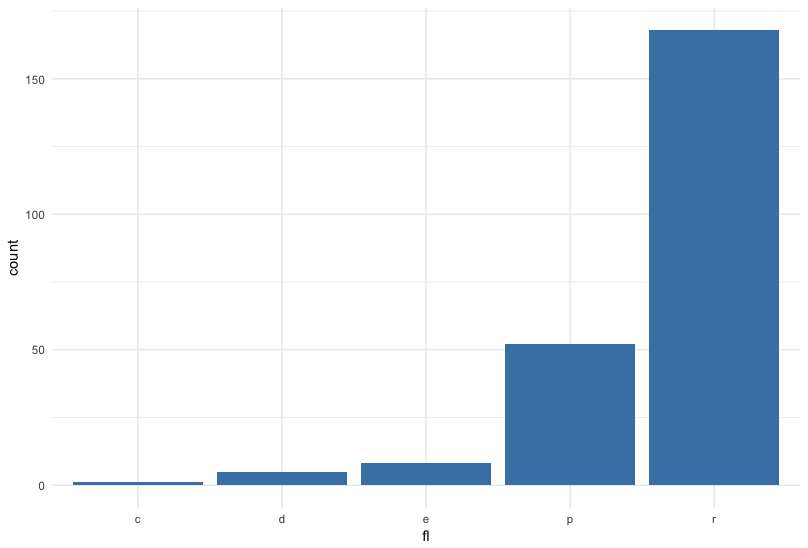
\includegraphics[scale=1 ]{ilu/bg34.png}\end{center}\end{figure}

\begin{figure}[H]\begin{center}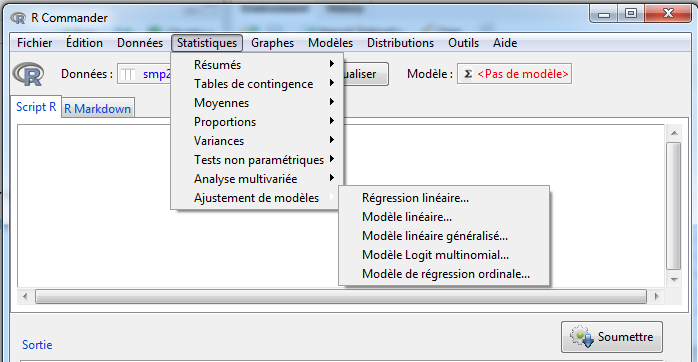
\includegraphics[scale=1 ]{ilu/bg.png}\end{center}\end{figure}




\begin{figure}[H]\begin{center}\includegraphics[scale=1 ]{ilu/.png}\end{center}\end{figure}


%% remplacer les ''''

\subsubsection{Exercice 5}
Créer dans R la fonction $f : \mathbb{R}^{n} \times \mathbb{R}^{n}$ définie par :
$$f(m,n)=\sum_{k=1}^{n} k^{m}$$



\subsubsection{Exercice 7}
Créer dans R la fonction $f : \mathbb{R}^{n} \times \mathbb{R}^{n}$ définie par :
$$f(x_{1},\dots,x_{n}) = \left(x_{1},\frac{x_{2}^{2}}{2},\dots,\frac{x_{n}^{n}}{n}\right)$$

\subsubsection{Exercice 9}
Créer dans R la fonction $f : \mathbb{N}^{2} \times [0;1] \rightarrow [0; 1]$ définie par :
$$f(k,n,p) = \binom{n}{k}p^{k}(1-p)^{n-k}$$